\RequirePackage{xcolor}
\documentclass[a4paper,11pt]{article}

\input{commands.tex}
\usepackage{tikz,algorithm,algpseudocode,diagbox}
\usepackage{natbib,filecontents}
\usetikzlibrary{arrows, shapes, calc, positioning}

\begin{filecontents}{reference.bib}
@book{witten1999managing,
  title={Managing gigabytes: compressing and indexing documents and images},
  author={Witten, Ian H and Witten, Ian H and Moffat, Alistair and Bell, Timothy C and Bell, Timothy C and Bell, Timothy C},
  year={1999},
  publisher={Morgan Kaufmann}
}
@misc{nelson2014data, 
    title={Data Compression With Arithmetic Coding}, 
    url={https://marknelson.us/posts/2014/10/19/data-compression-with-arithmetic-coding.html}, 
    author={Mark Nelson}, 
    year={2014}, 
    month={Oct}
}
\end{filecontents}

\begin{document}
\title{Coding Methods in Text Compression}
\author{Yanhua Huang}
\date{Mar 2020}
\maketitle

In this post, we review coding methods in text compression, with the assumption that the reader has a basic knowledge of data structures and algorithms, such as heap, prefix tree, and Huffman coding.

\section{Background}

\begin{figure}
\begin{center}
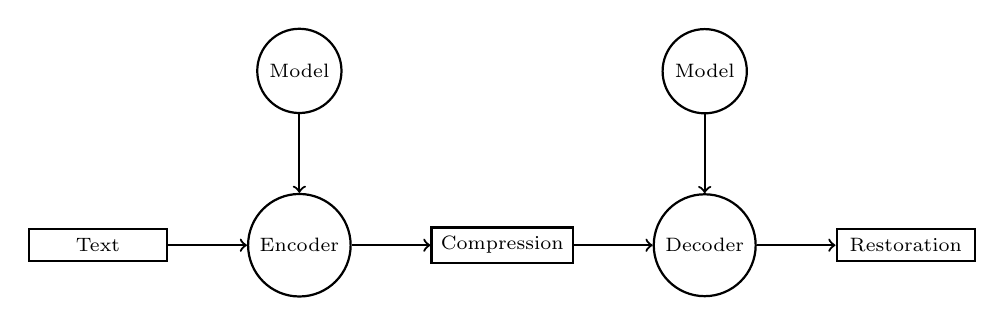
\begin{tikzpicture}{node distance=3cm, >=stealth}
\draw
    node [draw, thick, minimum width=5em] (input) {\scriptsize{Text}}
    node [circle, draw, thick, minimum size=3em, right=of input] (encoder) {\scriptsize{Encoder}}
    node [circle, draw, thick, minimum size=3em, above=of encoder] (model1) {\scriptsize{Model}}
    node [draw, thick,  minimum width=5em, right=of encoder] (compression) {\scriptsize{Compression}}
    node [circle, draw, thick, minimum size=3em, right=of compression] (decoder) {\scriptsize{Decoder}}
    node [circle, draw, thick, minimum size=3em, above=of decoder] (model2) {\scriptsize{Model}}
    node [draw, thick,  minimum width=5em, right=of decoder] (restoration) {\scriptsize{Restoration}}
;
\draw[->, thick] (input.east) -- (encoder.west); 
\draw[->, thick] (model1.south) -- (encoder.north); 
\draw[->, thick] (encoder.east) -- (compression.west); 
\draw[->, thick] (compression.east) -- (decoder.west); 
\draw[->, thick] (decoder.east) -- (restoration.west); 
\draw[->, thick] (model2.south) -- (decoder.north); 
\end{tikzpicture}
\end{center}
\caption {A general pipeline of text compression and restoration~\citep{witten1999managing}.}
\label{fig:general_pipeline}
\end{figure}

Compression is a kind of space-time tradeoff technique. A typical application scenario is the client/server computing, where compression saves storage in the server and reduce the network transmission, but takes more time on the client to decompress. Fig.~\ref{fig:general_pipeline} shows a general compression pipeline for text, where model provides distribution of symbols, and coding determines the compressed representation, also known as the codeword, of the symbol. For example, in Huffman coding, the model consists of the probabilities of each character, and the encoder (decoder) maps the texts (bits) to bits (texts). 

There are numbers of modeling and coding methods with different advantages. To design an appropriate pipeline in a specific scene, we need to consider three aspects. The first one should be the compression ratio, which is the bottleneck of space-saving. The second one is the speed of decoding, which determines how much time we will spend on decompression. The last one is the overhead for decoding individual documents, which is important for multi-documents situation. 

The simplest model that views symbols as independent and static random variables is difficult to satisfy the requirements above. There are two main ways to expand the model. On the one hand, the model can adapt to the text as the compression incrementally. On the other hand, the model can consider the distribution with the context. Most of the modern compression softwares utilize two expansions at the same time, e.g., an adaptive prefix tree is built to store the context dictionary in PDF.

The general idea of coding methods is that the lower the frequency of symbols, the fewer bits their codewords should occupy. There are two major classes of coding methods, the Huffman coding, and the arithmetic coding. In the rest of this post, we first introduce a well-known improvement over the standard Huffman code, known as canonical Huffman code, and then discuss the arithmetic code that can achieve a better compression ratio than Huffman codes in some cases.


\section{Canonical Huffman Code}
A Huffman code is an optimal prefix code that is widely used in lossless data compression. However, in standard Huffman coding, the Huffman tree is a big overhead. On the one hand, it takes much space to store internal nodes and pointers for the tree structure, especially in situations with many rare symbols. On the other hand, it is inefficient to jump randomly through the tree to parse the input bit one by one during decompression. 

Note that a Huffman code represents a prefix-free assignment of codewords where the length of each codeword is equal to the depth of the corresponding symbol in a Huffman tree. In other words, there may exist a regular relabeling method that can achieve a more efficient reassignment. Canonical Huffman code follow this idea and achieve less storage as well as faster decompression, where ``canonical'' means minimual randomness, e.g., exchanging the role of 0 and 1, or changing the combination order of nodes with the same weight leads to a different result but is equally valid. Canonical Huffman code are commonly used in many applications, such as PNG, JPEG, and MPEG. We describe the process of canonical coding in detail below.

In the encoding procedure, first of all, symbols are sorted in decreasing order by the bit length calculated with standard Huffman's algorithm, where symbols with the same bit length are sorted lexicographically in increasing order. We mark the sorted symbols with their bit lengths as $\{(s_i, l_i)\}_{i=1}^n$, where $s_i$ is the $i$-th symbol and $l_i$ is the corresponding bit length. The canonization is shown as in Alg.~\ref{alg:chc_encoding}. Note that we can further speed up the first step in the encoding procedure by only calculating depths of nodes instead of a whole tree with the help of a min-heap.

\begin{algorithm}[h] 
\caption{Encoding symbols by canonical Huffman coding.} 
\begin{algorithmic}[1]
\State $c_1 \leftarrow 0 << (l_1 - 1)$
\For{$i = 2, ..., n$}
\State $c_i \leftarrow (c_{i-1} >> (l_{i-1} - l_i)) + 1$
\EndFor
\State \Return $\{c_i\}_{i=1}^n$
\end{algorithmic} 
\label{alg:chc_encoding}
\end{algorithm}

There are two obvious properties of canonical Huffman code, which makes random access and contiguous storage available. The first one is that codewords with the same length are continuous and incremental numerically. The second one is that for any pair of codewords $x$ and $y$ with length $|x| > |y|$, $y$ is greater than arbitrary prefix of $x$ with length $|y|$. In the decoding procedure, we can use the second property to know whether a leaf node is reached, and achieve random access by calculating the offset with the first property. The decoding algorithm is shown as Alg.~\ref{alg:chc_decoding}. 

\begin{algorithm}[h] 
\caption{Decoding a canonical Huffman code.} 
\begin{algorithmic}[1]
\State $l \leftarrow 0$
\State $v \leftarrow \mathrm{readNBits}(\mathcal{I}[l])$
\While{$v < \mathcal{F}[l]$}
\State $l \leftarrow l + 1$
\State $step \leftarrow \mathcal{I}[l]$
\State $v \leftarrow (v << step) + \mathrm{readNBits}(step)$
\EndWhile
\State \Return $\mathcal{S}[l][v - \mathcal{F}[l]]$
\end{algorithmic} 
\label{alg:chc_decoding}
\end{algorithm}

As a consequence, we can only store the following three arrays for each bit length instead of a Huffman tree for decompression. A one-dimensional array $\mathcal{F}$ to store first codewords of bit lengths. A one-dimensional array $\mathcal{I}$ to store gaps between consecutive bit lengths. A two-dimensional array $\mathcal{S}$ to store lexicographically ordered symbols. For example in Table~\ref{table:chc_example}, $\mathcal{F} = [1, 1, 0]$, $\mathcal{I} = [1, 2, 1]$, and $\mathcal{S} = [[a], [b, c, d], [e, f]]$.

\begin{table}[h]
\centering
\begin{tabular}{c|c|c|c}
Symbol & Standard Huffman code & Bit length & Canonical Huffman code \\
\hline
a & 0    & 1 & 1 \\
b & 100  & 3 & 001 \\
c & 101  & 3 & 010 \\
d & 111  & 3 & 011 \\
e & 1100 & 4 & 0000 \\
f & 1101 & 4 & 0001
\end{tabular}
\caption{An example of canonical Huffman code.} 
\label{table:chc_example}
\end{table}


\section{Arithmetic Coding}
Consider the text containing two symbols only: $a$ and $b$ with probability $0.999$ and $0.001$, respectively. By Huffman coding, the expected length of codeword is 1 which is far less than the entropy of the text. The problem is that the Huffman codes force the bits of codewords to round up to integers. The arithmetic coding addresses this issue by aggregating fractional bits.

More precisely, the idea of the arithmetic coding is to encode a string as a unique real number in $[0, 1]$. In particular, given symbols $\{s_i\}_{i=1}^{n}$ and their probabilities $\{p_i\}_{i=1}^{n}$, we first divide $[0, 1]$ into $n$ subintervals, with the length of the $i$-th subinterval equal to $p_i$. Then, we divide each subiterval in the same way recursively, which just like construct a segment tree from top to bottom for all possible strings. Lastly, we output arbitrary float number in the final interval. In decoding procedure, by finding the interval that the given real number belongs to, we can restore the raw string. It is obvious that the length of the final subinterval is equal to the product of the probabilities of the symbols in the string, which is the probability of the string in the text. Note that we need $\log n$ more bits to store the length of the string, which is necessary for the decoder to know the stopping time. 

There are some numerical stability issues in arithmetic coding, e.g., for infinite strings, we require a float with infinite precision. Next, we start with a simple example and then discuss these problems with the C++ example. For unbounded precision, if the current interval is $[0.7530, 0.7599)$, it is obvious that the final float number must have the prefix $0.75$. As a result, we can output the longest common prefix of the current interval, i.e., $0.75$, and then consider the rest interval $[0.30, 0.99)$ in the next step. The implementation of arithmetic coding is shown as follows~\citep{nelson2014data}.

\begin{lstlisting}[language=C++]
// Input Model
unsigned int[] cumulativeFrequency;
unsigned int totalFrequency;

// Initialization
unsigned int ub = 0xFFFFFFFFU;    // $\underbrace{1...1}_{32}$
unsigned int lb = 0;              // $\underbrace{0...0}_{32}$
unsigned int b11 = 0xC0000000U; // $11\underbrace{0...0}_{30}$
unsigned int b10 = 0x80000000U; // $1\underbrace{0...0}_{31}$
unsigned int b01 = 0x40000000;  // $01\underbrace{0...0}_{30}$
char s;
int cache = 0;

// help function
void output_with_cache(bool bit, int &cache) {
	cout << bit;
	while (cache--)
		cout << !bit;
}

// Iteration
while (inStream >> s) {
	int range = ub - lb + 1;
	ub = lb + (range * cumulativeFrequency[s+1]) / totalFrequency;
	lb = lb + (range * cumulativeFrequency[s]) / totalFrequency;

	while (true) {
		if (ub < b10) {	         // [0xxxx, 0xxxx)
			output_with_cache(0);
			lb <<= 1;
			ub = (ub << 1) | 1;  // append precision
		} else if (lb >= b10) {	 // [1xxxx, 1xxxx)
			output_with_cache(1);
			lb <<= 1;
			ub = (ub << 1) | 1;  // append precision
		} else if (lb >= b01 && ub < b11) {
			// [01xxx, 10xxx) this is the case where the ub is closed to the lb
			cache++;  // cache the number and then correct the precision
			lb = (lb << 1) & 0x7FFFFFFF;  // $0\underbrace{1...1}_{31}$
			ub = (ub << 1) | 0x80000001; // $1\underbrace{0...0}_{30}1$
		} else { // [00xxx, 10xxx) or [00xxx, 11xxx) or [01xxx, 11xxx]
			// need a closer lb and ub to determine the common prefix
			break;
		}
	}
}
\end{lstlisting}

\bibliographystyle{plainnat}
\bibliography{reference} 

\end{document}